\chapter{Kiểm thử và đánh giá}\label{chap:danhgia}

\section{Chiến lược kiểm thử}
\begin{table}[H]
\centering\small
\caption{Các tầng kiểm thử}\label{tab:kiemthu}
\begin{tabularx}{\linewidth}{@{}lXl@{}}
\toprule
\textbf{Tầng} & \textbf{Nội dung} & \textbf{Khi chạy} \\ \midrule
Nhẹ & Cấu hình, API, lớp truy cập Cassandra, phát lại, dashboard; Cassandra được giả lập ở tầng driver nhưng giữ đúng cách ghi đè theo khóa & Mỗi lần sửa code, vài giây \\
Hồi quy contract & Mô tả API công bố phải trùng bản đã lưu; cột của lược đồ Cassandra phải trùng các trường lớp truy cập kiểm tra; từ điển dữ liệu phải liệt kê đủ bảng & Cùng tầng nhẹ \\
Spark & Các phép biến đổi và cách điều phối truy vấn, chạy trong container có Java & Khi sửa phần xử lý \\
Tích hợp & Lớp truy cập trên Cassandra thật, keyspace ngẫu nhiên, tự xóa sau khi chạy & Khi sửa lược đồ, truy vấn \\
End-to-end & Dựng hệ thống riêng, phát dữ liệu mẫu hai pha, kiểm tra cả ba tầng, API và giao diện & Trước khi nghiệm thu \\
\bottomrule
\end{tabularx}
\end{table}
Lệnh chạy từng tầng ở Phụ lục~\ref{app:ma}. Tầng hồi quy contract giúp thay đổi giao diện không lọt qua âm thầm.
Đổi tham số, trường trả về hay cột lưu trữ mà không cập nhật bản mô tả API đã lưu thì test thất bại. Người sửa vì thế
phải cập nhật cả bản mô tả lẫn contract của nhóm trong cùng một lần nộp.

\section{Kết quả CP0}
Dữ liệu mẫu ngày 01/01/2026 gồm 11 bản ghi. Kết quả chạy thật (Bảng~\ref{tab:cp0}) khớp bộ kết quả kỳ vọng; bộ này
được viết tay độc lập, không sinh ra từ chính code xử lý.

\begin{table}[H]
\centering\small
\caption{Kết quả CP0 trên dữ liệu mẫu, cửa sổ 2026-01-01 00:00 UTC}\label{tab:cp0}
\begin{tabularx}{\linewidth}{@{}Xr@{}}
\toprule
\textbf{Chỉ tiêu} & \textbf{Kết quả} \\ \midrule
Bản ghi Kafka / Bronze raw & 11 / 11 \\
Bronze invalid & 2 \\
Silver (sau loại trùng và canary) & 7 \\
Gold cửa sổ 00:00 (đã chốt) & 2 dòng \\
enwiki: event / edit / trang mới / ẩn danh / bot & 5 / 5 / 0 / 1 / 1 \\
viwiki: event / edit / trang mới / ẩn danh / bot & 1 / 0 / 1 / 0 / 0 \\
\bottomrule
\end{tabularx}
\end{table}

\begin{table}[H]
\centering\small
\caption{Các lần kiểm chứng}\label{tab:kiemchung}
\begin{tabularx}{\linewidth}{@{}llX@{}}
\toprule
\textbf{Ngày} & \textbf{Máy} & \textbf{Kết quả} \\ \midrule
11/10/2026 & Apple M3, ARM64 & 84 test nhẹ đạt; 16 test Spark đạt; kiểm thử end-to-end đạt (Trọng) \\
15/10/2026 & Windows 11, x86\_64 & CP0 chạy lại, số khớp Bảng~\ref{tab:cp0} (Thành) \\
22/10/2026 & Windows 11, x86\_64 & Bộ \code{api/tests} đạt 33 test; lượt Cassandra integration đạt 4 test (Nhân) \\
23/11/2026 & Windows 11, x86\_64 & 179 test nhẹ toàn repo, gồm 68 test API; một lượt riêng có 8 test Cassandra thật đạt; end-to-end ghi Cassandra khớp Bảng~\ref{tab:w2fixture} (Nhân) \\
23/11/2026 & Windows 11, x86\_64 & Hồi quy sau khi gộp: 183 test nhẹ đạt (gồm 4 test hồi quy contract); 8 test trên Cassandra thật đạt; kiểm thử end-to-end đạt; các lệnh vận hành serving chạy đúng trên hệ thống thật (Nhân) \\
\bottomrule
\end{tabularx}
\end{table}
\dukiensua{Mỗi thành viên chạy lại CP0 trên máy mình thì thêm một dòng (CP1).}

\begin{ghichu}{Bài học khi chạy trên Windows}
Hai lỗi chỉ xuất hiện trên Windows. (1) Git trên Windows mặc định đổi ký tự xuống dòng của file sang kiểu Windows (CRLF);
script tạo topic chạy trong container Linux vì thế đọc sai và dừng. Cách sửa: khai báo cho Git luôn giữ kiểu Linux (LF)
với mọi script shell. (2) Thư viện Cassandra cho Python cần một module đã bị gỡ khỏi Python 3.12; container dùng
Python 3.11 nên không bị, còn máy phát triển dùng 3.12 phải cài thêm gói thay thế. Bài học: mỗi thành viên nên chạy lại
toàn bộ hệ thống trên máy mình sớm (mốc CP1), vì lỗi môi trường không lộ ra khi chỉ chạy trên một máy.
\end{ghichu}

\section{Xu hướng và ưu tiên xem xét trên fixture vàng}
Ngày 23/11/2026, nhóm dựng một hệ thống riêng với Spark ghi cả ba nghiệp vụ mới vào Cassandra, phát lại toàn bộ 11 bản ghi
mẫu rồi hỏi qua API. Cả chín truy vấn Spark đều chạy. Mọi số liệu API trả về (Bảng~\ref{tab:w2fixture}) trùng với bộ
kỳ vọng viết tay độc lập mà phần xử lý dùng để kiểm tra đầu ra Parquet. Như vậy cùng một kết quả đi qua được cả hai
đường lưu: Parquet và Cassandra.

\begin{table}[H]
\centering\small
\caption{Kết quả qua API trên dữ liệu mẫu (enwiki)}\label{tab:w2fixture}
\begin{tabularx}{\linewidth}{@{}Xr@{}}
\toprule
\textbf{Chỉ tiêu} & \textbf{Kết quả} \\ \midrule
Chi tiết sự kiện lưu trong Cassandra & 7 (bằng số sự kiện Silver) \\
Cửa sổ 00:00--00:05, trang 10: chỉnh sửa / người sửa / byte thay đổi / điểm & 4 / 3 / 1.890 / 0,12475 \\
Cửa sổ 00:00--00:05, trang 11: chỉnh sửa / người sửa / byte thay đổi / điểm & 1 / 1 / 5 / 0,022625 \\
Chỉnh sửa cần ưu tiên: xóa nhiều nội dung / hoàn tác / sửa ẩn danh & điểm 30 / 20 / 10 \\
Sự kiện không dính dấu hiệu nào & điểm 0, không có lý do \\
Định danh không tồn tại & lỗi \enquote{không tìm thấy sự kiện} \\
\bottomrule
\end{tabularx}
\end{table}
Các số trong bảng là kết quả API của cửa sổ provisional 00:00--00:05 ở lần chạy của Nhân. Ở một phép kiểm khác,
Linh ghi nhận Gold finalized cho cửa sổ 23:56--00:01 của ngày hôm trước, với cùng các giá trị trend score trên fixture;
hai kết quả thuộc hai đầu ra và hai cửa sổ khác nhau. Giá trị số người sửa dùng phép ước lượng
\code{approx\_count\_distinct}, không phải cam kết đếm chính xác cho mọi tập dữ liệu.
\dukiensua{Thêm ảnh chụp trang Trending, Suspicious Edits khi W2-MANH-01 xong.}

\section{Độ trễ end-to-end}\chualam
\section{Khởi động lại, retry và dữ liệu đến muộn}
Retry được kiểm tra cho cả bốn loại dữ liệu phục vụ: hoạt động và xu hướng trên Cassandra thật (keyspace tạm, xóa sau
khi chạy), chỉnh sửa cần ưu tiên và chi tiết sự kiện trên bản giả lập ở tầng driver vốn giữ đúng cách ghi đè theo khóa.
Ghi cùng một dòng hai lần, rồi ghi lại với giá trị mới, thì mỗi khóa vẫn chỉ có một dòng mang giá trị mới nhất. Ghi lại các
batch xu hướng không tạo thêm cửa sổ trong chỉ mục. \enquote{Cửa sổ mới nhất} lấy từ chỉ mục luôn là cửa sổ vừa ghi.
Danh sách lý do rỗng đọc ra đúng là rỗng, không thành giá trị trống. Truy vấn theo khoảng phút chạy được mà không cần
cho phép quét bảng.
Lượt kiểm thử W3 của Linh ngày 08/11/2026 dùng Kafka, Spark, HDFS và Cassandra activity trong môi trường cô lập.
Fixture lần lượt đưa duplicate, late event, event làm watermark tiến và event quá muộn vào hệ thống. Bảy trong bảy
phase đạt, chín Spark query giữ query ID qua JVM mới nhờ checkpoint. Đầu ra cuối gồm 13 Bronze raw, 2 Bronze invalid,
6 Silver, 2 suspicious edit, 2 dòng Gold activity và 10 dòng Gold trends. Bronze raw và invalid là hai nhánh
có thể chồng lấp nên không cộng số dòng của chúng thành tổng. Gold được quan sát sau khi event time tiến watermark,
không kết luận rằng chỉ chờ thời gian thực là đủ chốt cửa sổ. Analytics trong lượt này ghi Parquet; kết quả không
chứng minh LIVE end-to-end hoặc exactly-once giữa các sink. Nguồn: \code{docs/plans/W3-LINH-01.md}.

Trong phép thử W3 của Trọng, hệ thống lưu kết quả REPLAY, dừng Spark rồi tạo lại Kafka, Cassandra và HDFS với volume
cũ. API đọc activity khi Spark vẫn dừng, sau đó Spark được khởi động lại từ checkpoint. Trình tự này giúp phân biệt
dữ liệu Cassandra đã còn qua restart với dữ liệu có thể được Spark ghi lại sau restart. Phép thử thuộc REPLAY và
cấu hình riêng được ghi tại \code{docs/plans/W3-TRONG-01.md}; không suy ra mọi kịch bản lỗi đều được bao phủ.

\begin{figure}[H]
\centering
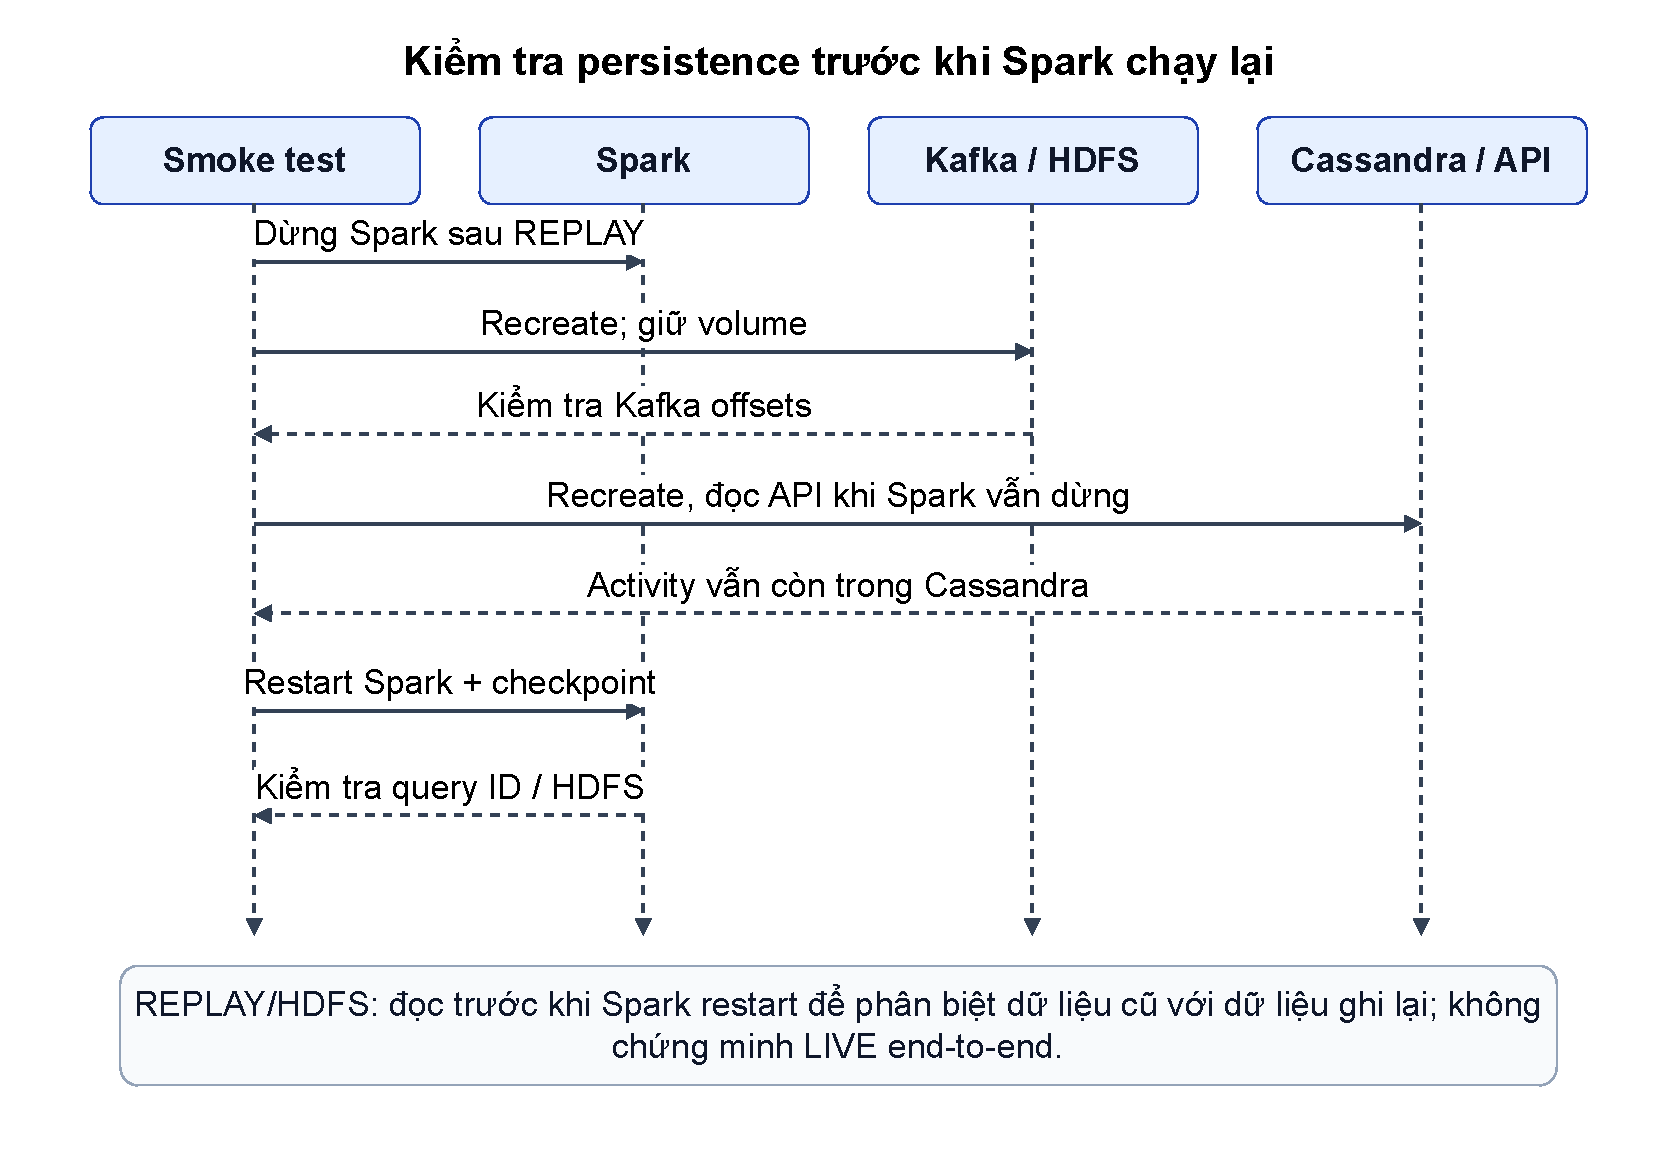
\includegraphics[width=\linewidth]{so-do/seq-recovery.pdf}
\caption{Một kịch bản kiểm thử REPLAY/HDFS: đọc API khi Spark còn dừng giúp kiểm tra dữ liệu Cassandra tồn tại qua restart, trước khi Spark có thể ghi lại.}\label{fig:recovery-sequence}
\end{figure}

Một bài đo W3 khác của Thành gửi 1.200 event tổng hợp dùng cùng key, sau đó khởi động lại Spark. Ba query
\code{bronze\_raw}, \code{bronze\_invalid} và \code{silver\_events} báo input end-offset đạt đích khi được
quan sát ở 8,984 giây sau khi gửi xong; phép đo gồm thời gian khởi động lại và polling. Con số không phải độ trễ
tới API/dashboard, cũng không phải benchmark cho nhiều partition. Nguồn: \code{docs/plans/W3-THANH-01.md}.

\section{Chạy LIVE liên tục}
Ngày 23/11/2026, Thành chạy collector LIVE trong Docker Compose trên Windows trong khoảng 20 phút 45 giây;
collector nhận và ghi nhận ACK liên tiếp cho 40.112 event, với sáu reconnect, không ghi nhận parse error hay
publish failure trong counter. Mạng collector được ngắt có chủ đích 75 giây và số ACK tiếp tục tăng sau khi kết nối lại.
Nguồn: \code{docs/plans/W2-THANH-01.md}.

Cùng ngày, một lượt trên EC2 \code{m7i-flex.large} chạy 30 phút 44 giây. Collector ghi nhận 70.252 event nhận,
70.252 event đã publish, năm reconnect, không restart, \code{parse\_errors=0} và \code{publish\_failed=0}; tổng
Kafka end-offset là 70.252. Counter parse chỉ đếm JSON sai hoặc không phải object, không xác nhận toàn bộ schema.
Sự tương ứng giữa counter và tổng offset không đối chiếu ID duy nhất và không chứng minh không mất/trùng end-to-end.
Smoke REPLAY core trên EC2 đạt tám kiểm tra, không chạy HDFS. Máy dùng snapshot của working tree chưa commit vào
thời điểm thử, không phải clean clone từ commit. Tài nguyên thử đã được dọn. Nguồn:
\code{docs/plans/W4-THANH-01.md}. Các lượt này không tự đóng CP3 hoặc CP4.
\section{Tải và dung lượng}\label{sec:dungluong}
\dukiensua{Tải Spark và latency dưới tải: cần Linh bổ sung evidence.}
\subsection{Dung lượng Cassandra và hạn lưu chi tiết sự kiện}
Số đo lấy trên một node Cassandra 4.1.8 chạy trong Docker trên máy Windows 11. Công cụ đo ghi dữ liệu tổng hợp đúng cấu
trúc contract vào một keyspace tạm, qua cùng lớp truy cập mà Spark dùng. Sau đó công cụ ép Cassandra ghi xuống đĩa, đọc
dung lượng thật, rồi xóa keyspace (Bảng~\ref{tab:dungluong}).

\begin{table}[H]
\centering\small
\caption{Dung lượng và tốc độ ghi đo được}\label{tab:dungluong}
\begin{tabularx}{\linewidth}{@{}Xrrrr@{}}
\toprule
\textbf{Bảng} & \textbf{Dòng} & \textbf{Byte trên đĩa} & \textbf{Byte/dòng} & \textbf{Dòng/giây} \\ \midrule
Chi tiết sự kiện & 20.000 & 2.890.920 & 144,5 & 78 \\
Xu hướng (một cửa sổ) & 5.000 & 84.194 & 16,8 & 79 \\
\bottomrule
\end{tabularx}
\end{table}

Hai dòng của bảng đo hai thứ khác nhau. Dòng đầu là số sự kiện, quyết định hạn lưu. Dòng thứ hai là một cửa sổ xu hướng
đúng bằng giới hạn 5.000 trang, dùng để kiểm tra rằng đọc cả partition lớn nhất được phép vẫn nhanh: lấy top-20 mất
156~ms. Dữ liệu tổng hợp lặp lại nhiều nên nén tốt hơn dữ liệu thật; số byte của bảng xu hướng chỉ để thấy partition
nhỏ, không dùng để ước tính.

Mẫu W1 có khoảng 2,3 event/giây cho hai wiki, tương đương 200.000 event/ngày. Với 145 byte/dòng, ước tính
29~MB/ngày hoặc 200~MB cho 7 ngày; hạn lưu event detail được chọn là 7 ngày. Tốc độ 78 dòng/giây đo trên một node với
fixture tổng hợp không chứng minh khả năng xử lý ổn định tải LIVE toàn cầu.

% ============================================================================
% CHƯƠNG 6: KẾT LUẬN
% ============================================================================
